\chapter{Results}
\label{chap:Results}

Below is the path followed by a randomly selected particle with initial energy $E=10^{14}$eV:

\begin{figure}[H]
    \includegraphics[width=0.88\textwidth]{Figures/example_random_walk.pdf}
    \centering
    \caption{Magnitudes of the 3D random walk of a random particle $(\theta_{\max}=\pi, \alpha=0)$. The blue arrow indicates the last position is located outside the graph in said direction. Also represented are the energy of the particle in each step and the interaction length of every step. When this last one becomes bigger than $R_c$, the particle inevitably escapes.}
    \label{fig:example_random_walk}
\end{figure}

The energy of the particle gets reduced exponentially in every collision (a straight line in logarithmic representation). The final energy is expected to be close to $E_\text{final} = E_\text{initial}\cdot 0.5^{N_{\text{int}}}$, $N_\text{int}$ being the number of interactions. Now, after binning the particles logarithmically according to their energy, we can build the simulated SED. The following plot shows the SED of NGC 1068's AGN for example values of the coronal radius, alpha and the maximum turning angle:

\begin{figure}[H]
    \includegraphics[width=\textwidth]{Figures/example_simulation_plot.pdf}
    \centering
    \caption{Spectral Energy Distribution of NGC 1068's AGN for $R_c=25R_s$, $\alpha=0.4$ and $\theta_{\max} = \pi$. The purple line represents the 10-year data from IceCube, as well as our initial flux for the photons. The blue dots are the simulated flux from the model. A polynomial of degree 5 has been fitted into the data. The 95\% confidence interval from the fit is also represented. Finally, the 4-year data from Fermi-LAT is represented as the black dots and upper limits.}
    \label{fig:example_simulation_plot}
\end{figure}

These are the results of the simulation for said values of the coronal radius, alpha and the turning angle, which are within reasonable expectation of the real values. However, it is also interesting to examine what the results of the model are for other values of $R_c$, $\alpha$ and $\theta_{\max}$. This way, we can check whether there is a combination of these parameters which produces results that better fit the data from Fermi-LAT:

\begin{figure}[H]
    \includegraphics[width=\textwidth]{Figures/simulations_plot.pdf}
    \centering
    \caption{Spectral Energy Distribution of NGC 1068's AGN for different values of $R_c/R_s$, $\alpha$ and $\theta_{\max}$. The purple line represents again the data from IceCube and our initial flux for the photons. The red, blue and yellow symbols represent the flux for different values of $\theta_{\max}$. The 4-year data from Fermi-LAT is represented as the black dots and upper limits.}
    \label{fig:simulations}
\end{figure}

One interesting takeaway from this plot is that $\theta_{\max}$ has very little influence in the results. Beamed particles tend to have slightly higher energies due to the fact that they're prone to taking fewer steps when cascading. However, there is practically no difference between the particles executing a complete random walk and being beamed. This is due to the fact that the last step of the random walk is the one which matters the most: particles can take as many steps as they want, but if the last step's length is larger than the coronal radius, it will be the one which determines the final energy of the particle. Thus, the maximum turning angle of the particles has been neglected in the rest of the analysis, assuming it is equal to $\pi$ (isotropic random walk).

These simulations are quite resource- and time-intensive. In order to find which parameters yield a better fit to the Fermi-LAT data, it is not practical to run the simulation for every possible combination of the parameters. Instead, we can use a machine learning algorithm to find the best fit. The idea is to use the simulated spectra as a training set for the algorithm, which will then be able to predict the shape of the spectrum given a certain combination of $R_c$ and $\alpha$\footnote{Since the maximum turning angle's effect has been shown to be negligible, I will simply assume the spectrum depends on said two parameters}, effectively ``interpolating'' between the data:

\begin{figure}[H]
    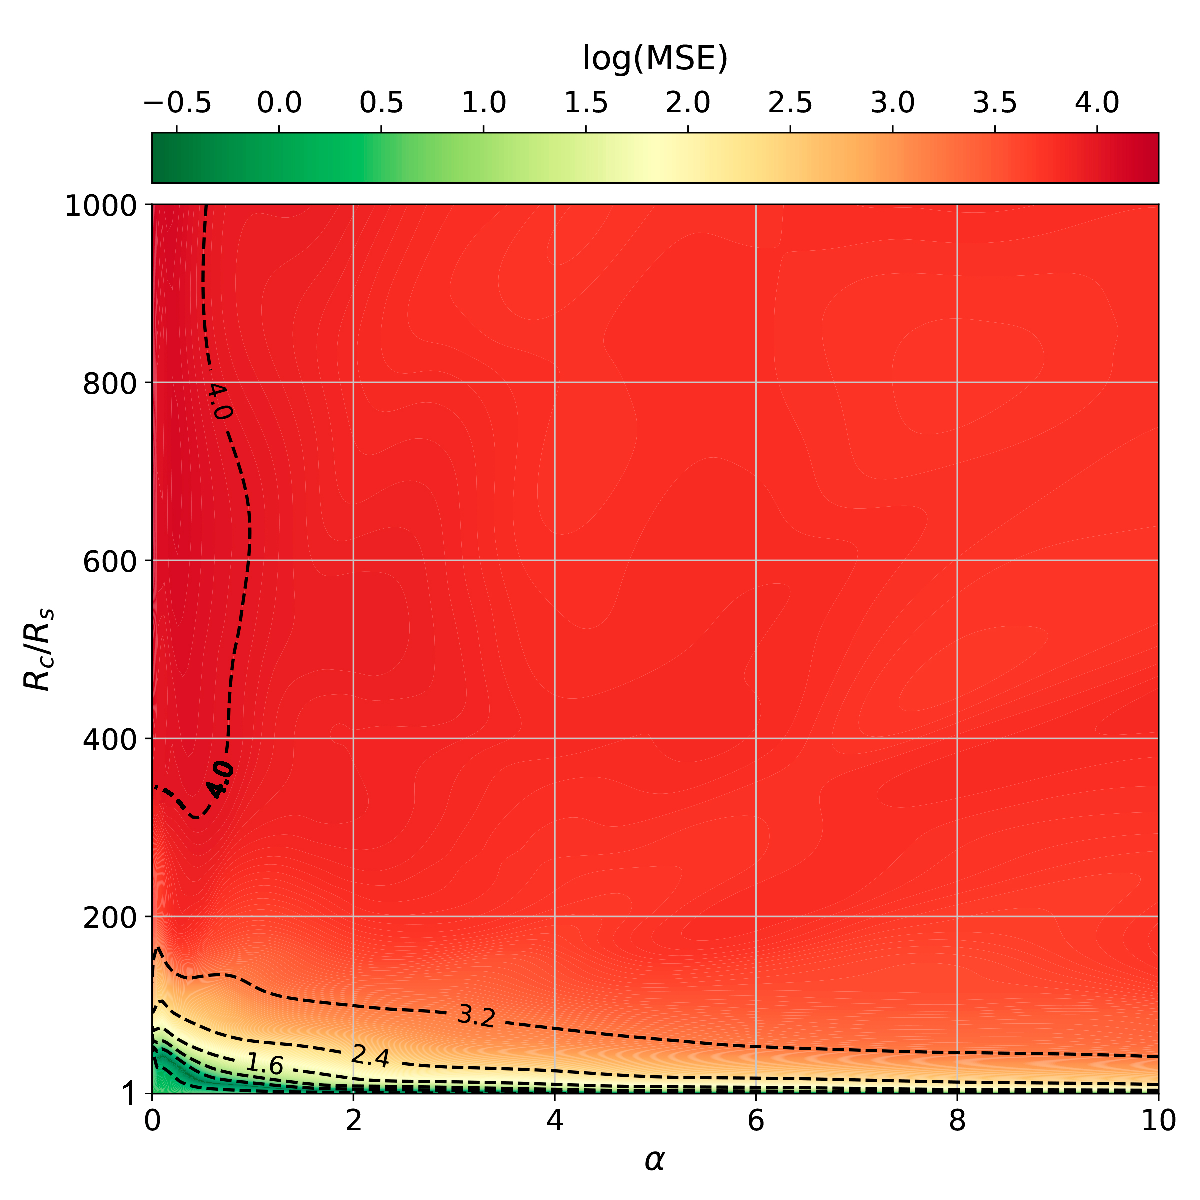
\includegraphics[width=0.9\textwidth]{Figures/10x1000_contour_plot.pdf}
    \centering
    \caption{Goodness of fit as a function of $\alpha$ and $R_c/R_s$. The color scale represents the logarithm of the MSE (mean squared error) of the fit. In order to reduce noise from the neural network, the MSE has been averaged over 20 different runs.}
    \label{fig:contour_plot_10x1000}
\end{figure}

Figure \ref{fig:contour_plot_10x1000} shows the goodness of fit for a large range of values of $R_c$. It can be seen that the MSE is very high regardless of $\alpha$ for $R_c/R_s$ values above 100. The most interesting part of the plot is thus the region $R_c/R_s \in [1, 60]$. Plotting said region in more detail, we can get a better idea of the shape of the MSE as a function of the parameters:
\begin{figure}[H]
    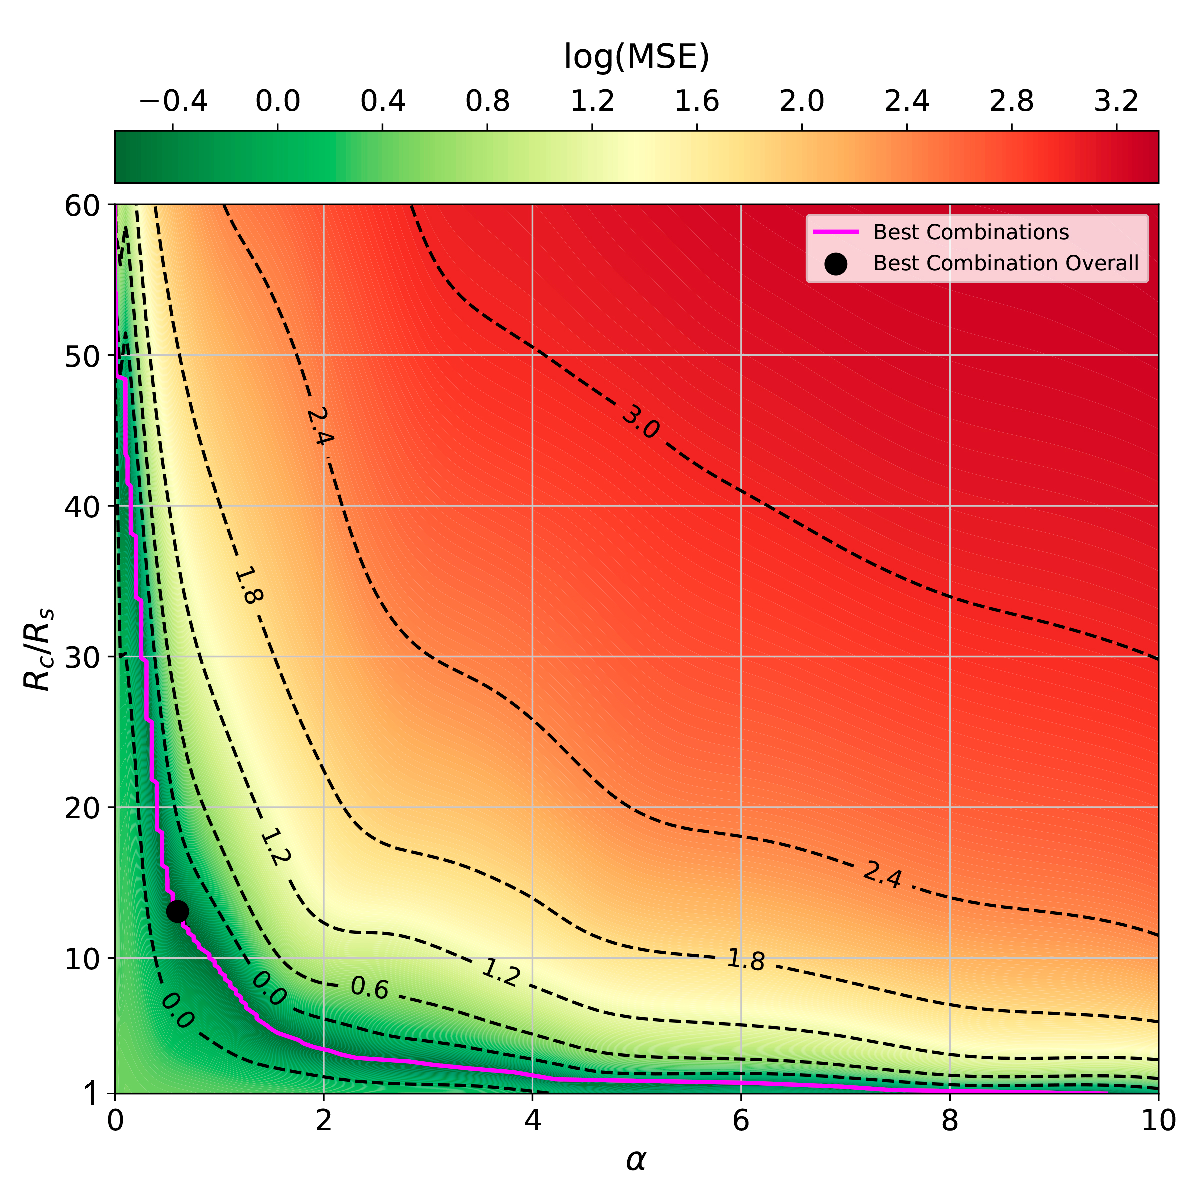
\includegraphics[width=0.9\textwidth]{Figures/10x60_contour_plot.pdf}
    \centering
    \caption{Goodness of fit as a function of $\alpha$ and $R_c/R_s$. The color scale represents the logarithm of the MSE of the fit. In order to reduce noise from the neural network even further, the MSE has been averaged over 30 different runs. Plotted are the best fits for each value of $\alpha$, as well as the best combination of parameters overall.}
    \label{fig:contour_plot_10x60}
\end{figure}

There is a very clear trade-off between the two quantities: either the corona is very small and the particles start towards its edge, or the corona is large, but the particles begin their cascades very close to the center. The best fit for the whole range of $\alpha$ is located at $R_c/R_s \approx 13$, $\alpha \approx 0.6$. This is consistent with the values estimated earlier for the coronal radius of NGC 1068. One can also see that the MSE starts to irreversibly increase for values of $R_c/R_s$ above 50, thus indicating that the coronal radius must not be larger than said value.

Now, all the different combinations of $R_c$ and $\alpha$ can be sorted by their MSE, and then simulated, to check whether the neural network is able to predict the shape of the spectrum correctly. The following plot shows the SED for the best fit, as well as the $1000$th, $3500$th, $5000$th up until the worst fit found by the algorithm:

\begin{figure}[H]
    \includegraphics[width=0.86\textwidth]{Figures/selected_simulations_plot.pdf}
    \centering
    \caption{Spectral Energy Distribution of NGC1068's AGN for the best fit, as well as $1000$th, $3500$th, $5000$th, up until the $430\,000$th. The purple line represents the data from IceCube (and our initial flux for the photons). The red line is the prediction from the neural network. Finally, the blue symbols represent the simulated flux. The 4-year data from Fermi-LAT is plotted as the black dots and upper limits. The legend shows the logarithm of the MSE of the fit, as well as the ordering of the simulations.}
    \label{fig:selected_simulations_plot}
\end{figure}

It is important to note that the MSE is not always a good measure of the goodness of fit. The prediction from the neural network has a noticeable ``tail'' at the end of the spectrum, which is not present in the simulated data. This is caused by the addition of synthetic data to the training set, in order to get the algorithm to train more accurately. This has the effect of creating artificial values in the prediction, which are not present in the simulated data. The result is that, for cases when $\alpha$ is very small, although the MSE is generally very high, it should be even higher. Take for example the $430\,000$th simulation. The MSE's logarithm has a value of $\sim 10$, however, no data is actually present in the tail of the spectrum. This means that the flux for that part of the spectrum would be zero, and thus, the MSE would tend towards infinity.

Finally, another way of checking which parameters yield the best fit is to check the frequency of the different combinations of $R_c$ and $\alpha$ whose MSE is below a certain threshold. The following plots show the frequency of the different combinations of $R_c$ and $\alpha$ whose MSE is below 0.3 and 1:

\begin{figure}[H]
    \includegraphics[width=0.89\textwidth]{Figures/Frequencymse0.30.pdf}
    \centering
    \caption{Heatmap of the frequency of the different combinations of $\alpha$ and $R_c/R_s$ whose MSE doesn't exceed 0.3. Boxed in black are the top four combinations whose frequency is the highest.}
    \label{fig:frequencymse0.3}
\end{figure}
\begin{figure}[H]
    \includegraphics[width=\textwidth]{Figures/Frequencymse1.pdf}
    \centering
    \caption{Heatmap of the frequency of the different combinations of $\alpha$ and $R_c/R_s$ whose MSE doesn't exceed 1. Boxed in black are the top nine combinations whose frequency is the highest.}
    \label{fig:frequencymse1}
\end{figure}

There are two main hotspots in these heatmaps: one at ($R_c/R_s \sim 10$, $\alpha \sim 0.8$), and another one at ($R_c/R_s \sim 3$, $\alpha \sim 2.3$). The first one is the same as the one found in the contour plots, while the second one is a bit more surprising. A coronal radius of $R_c/R_s \sim 3$ is very small, and would imply that the particles are starting very close to the center of the AGN. This is not consistent with the values found in the literature, which estimate the coronal radius to be at least $R_c/R_s \sim 10$. This suggests that the second hotspot might be an artifact of the model, or that the parameters are not well constrained in this region.

\section{Discussion}
\label{sec:Discussion}

The results presented in this chapter offer valuable insight into the potential conditions we could find in the AGN of NGC 1068, which have been inferred by comparing the simulated cascaded particle flux with data obtained from missions such as Fermi-LAT. While simple, the random walk model is capable of capturing the essential nature of the phenomena at hand, as well as the resulting exponential energy loss per collision, as illustrated in Figure \ref{fig:example_random_walk}. 

Comparing the simulated Spectral Energy Distributions (SEDs) with data from IceCube and Fermi-LAT (Figures \ref{fig:example_simulation_plot}, \ref{fig:simulations} and \ref{fig:selected_simulations_plot}) reveals the model's capability to reproduce the general trend of the observed gamma-ray flux at lower energies. An interesting result derived from the simulations is that of the low influence of the maximum turning angle, $\theta_{\max}$, which likely stems from the dominant influence of the final interaction step's length on the particle's escape energy. This observation justified neglecting $\theta_{\max}$ in the subsequent, more computationally intensive parameter space exploration, simplifying the problem to the connection between the coronal radius ($R_c$) and the initial distribution parameter ($\alpha$).

Given the computational demands of running full simulations for numerous parameter combinations, the machine learning approach proved essential. The contour plots derived from the neural network predictions (Figures \ref{fig:contour_plot_10x1000} and, more importantly, \ref{fig:contour_plot_10x60}) clearly delineate the valid parameter space. A distinct trade-off emerges between $R_c$ and $\alpha$: a smaller, more compact corona requires particles to start nearer the edge (higher $\alpha$) to match the observed spectrum, whereas a larger corona demands particles starting closer to the central source (lower $\alpha$) to undergo sufficient interactions. The region minimizing the Mean Squared Error (MSE) centers around $R_c/R_s \approx 13$ and $\alpha \approx 0.6$, which fits reasonably well with independent estimates for NGC1068's coronal radius found in the literature \citep{Eichmann_2022}.

The frequency analysis presented in Figures \ref{fig:frequencymse0.3} and \ref{fig:frequencymse1} further reinforces these findings. By mapping the density of parameter combinations yielding low MSE values, these heatmaps highlight the same preferred region identified in the contour plots, confirming the robustness of the best-fit parameters within the model's framework.

However, certain limitations must be acknowledged. The comparison between the neural network predictions and direct simulations (Figure \ref{fig:selected_simulations_plot}) revealed discrepancies, particularly the artificial "tail" in the predicted spectra at low energies for high MSE fits. This artifact, arising from the use of synthetic data during training, shows that the MSE, while a useful metric, may not perfectly capture the goodness-of-fit for different parameters, especially in regimes where the model performs poorly (e.g., very low $\alpha$). The true MSE in such cases might be significantly higher than calculated due to the sharp cutoff in simulated flux versus the predicted tail. It must also be acknowledged that although the simulations allow for the coronal radius to be just as small as the Schwarzschild radius, this is not a realistic assumption. The coronal radius ought to be larger than the Black Hole's event horizon. Otherwise, the particles wouldn't be able to escape the AGN at all.

% ... (rest of the template comments if needed) ...
% In this chapter, you describe the output from applying your methodology. Present your results in a clear manner, using a combination of figures and tables.

% If you are doing lab experiments: What do you observe? Also include qualitative observations that might not be directly relevant (“we saw more production at the upper half of the core sample than the lower half, with most production leaving at the upper side-plane”).

% If you are doing computations: What is the output from applying your code/software? Which part of your software is using the most computational power? How does it compare to other similar software?

% Illustrate the results. Use graphs, images, and tables (see Chapter \ref{chap:Theory}).

% A common challenge is to distinguish the results and the discussion section. Do not discuss your results in this chapter, that should be done in the discussion section. If it is hard to separate results and discussion, you might combine them into one section. You could also split the results and discussion part of your thesis into several results/discussion sections for different topics (“Magnesium effect on imbibition”, “Sodium effect on imbibition”).

% Try to avoid repetition between. In case you have many graphs of the same process, keep some characteristic graphs and move the rest to an appendix. Then you describe one graph in detail and refer to the others in the appendix for changes between the results.